\begin{center}
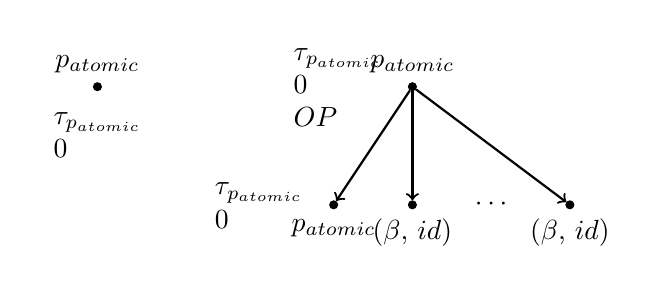
\begin{tikzpicture}[yscale=-1,
place/.style={circle,draw=black, fill=black, inner sep=0pt, 
              minimum size=1mm}]

	\node[place] (1st) at (1, 0) [label=above: $p_{atomic}$,
                                      label=below:
            \begin{tabular}{l}
              $\tau_{p_{atomic}}$\\
              $0$\\
            \end{tabular}] {};

\begin{scope}[xshift=4cm]
  \node[place] (1st) at (1, 0) [label=above: $p_{atomic}$,
                                label=left: 
             \begin{tabular}{l}
              $\tau_{p_{atomic}}$\\
              $0$\\
              $OP$\\ 
             \end{tabular}
] {};
	\node[place] (2nd) at (0, 1.5) [label=below: $p_{atomic}$,
                                        label=left: 
             \begin{tabular}{l}
              $\tau_{p_{atomic}}$ \\
              $0$ \\
             \end{tabular}
]{};
        \node[place] (3rd) at (1, 1.5) [label=below: {($\beta$, $id$)}] {};
	\node[place] (4rd) at (3, 1.5) [label=below: {($\beta$, $id$)}] {}; 

	\node (dots) at (2,1.5) {$\cdots$};
	
	\draw[->, thick] (1st) -- (2nd);
	\draw[->, thick] (1st) -- (3rd);
        \draw[->, thick] (1st) -- (4rd);
\end{scope}


\end{tikzpicture}
\end{center}   